We evaluate the proposed approach using a set of four experiments.
A toy problem is first used to study the transfer of learning between two related processes through the shared inducing points.
We then compare the model with existing multioutput models on the tasks of predicting foreign exchange rates and air temperature.
In the final experiment, we test the model on the prediction of robot arms dynamic on a large-scale dataset. 
All experiments are executed on an Intel(R) Core(TM) i7-2600 3.40GHz CPU with 8GB of RAM using Matlab R2012a.
%except for large scale?

\subsection{TOY PROBLEM}
In this toy problem, two related outputs are simulated from the same latent function $sin(x)$ corrupted by independent noises: $y_1(x) = sin(x) + \epsilon$ and $y_2(x) = -sin(x) + \epsilon$, $\epsilon \sim \Normal(0,0.01)$.
The first output has missing observations in the $(-7,-3)$ interval and the second output in the $(4,8)$ interval.
The predictive distributions by our model ($Q = 1$) and independent stochastic GPs (one for each output) are shown in \ref{fig:toy}.
It can be seen that our multioutput model gives perfect prediction in the unobserved regions where the independent models fail to interpolate despite having the same set of inducing inputs.
This confirms that transfer of information from one output to another via collaborative learning of the posterior over the shared inducing inputs.
Furthermore, the inference procedure learned that the weights are $w_{11} = 1.07$ and $w_{21} = -1.06$ which precisely reflects the correlation between the two outputs.

\begin{figure*}
\centering
\begin{tabular}{cccc}
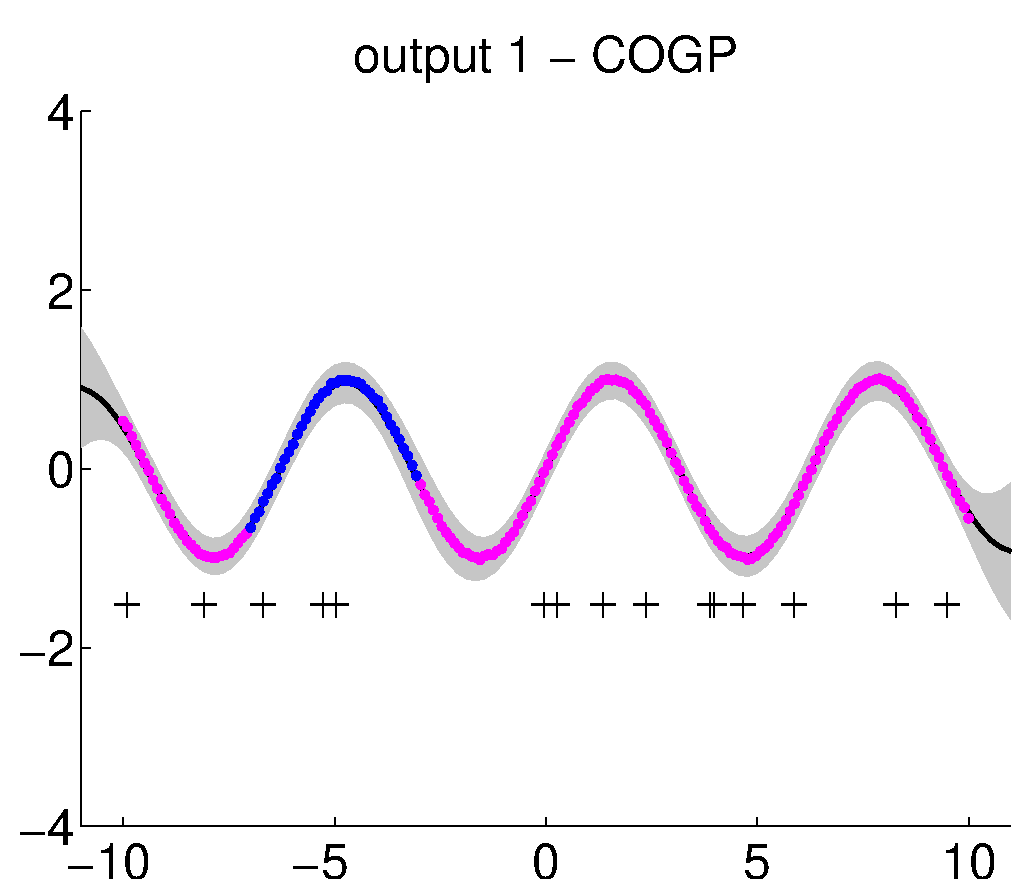
\includegraphics[scale=0.2]{figures/toy-slfm-y1.eps} &
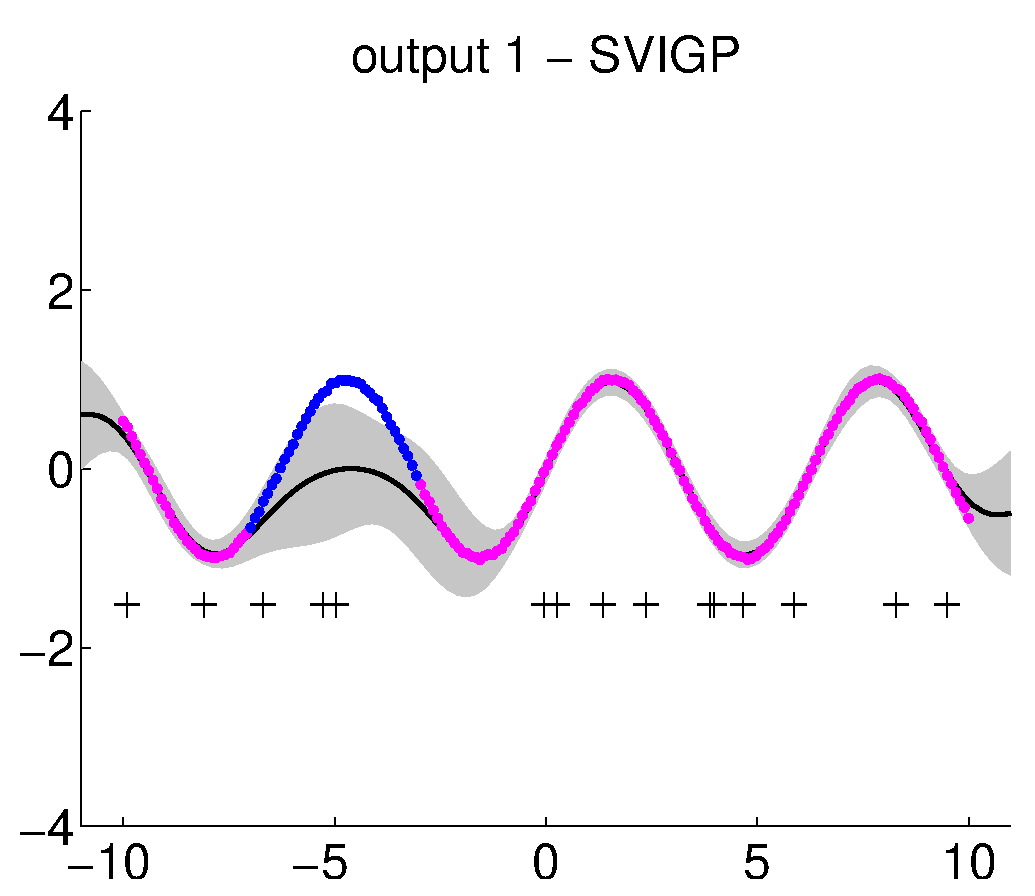
\includegraphics[scale=0.2]{figures/toy-svigp-y1.eps} &
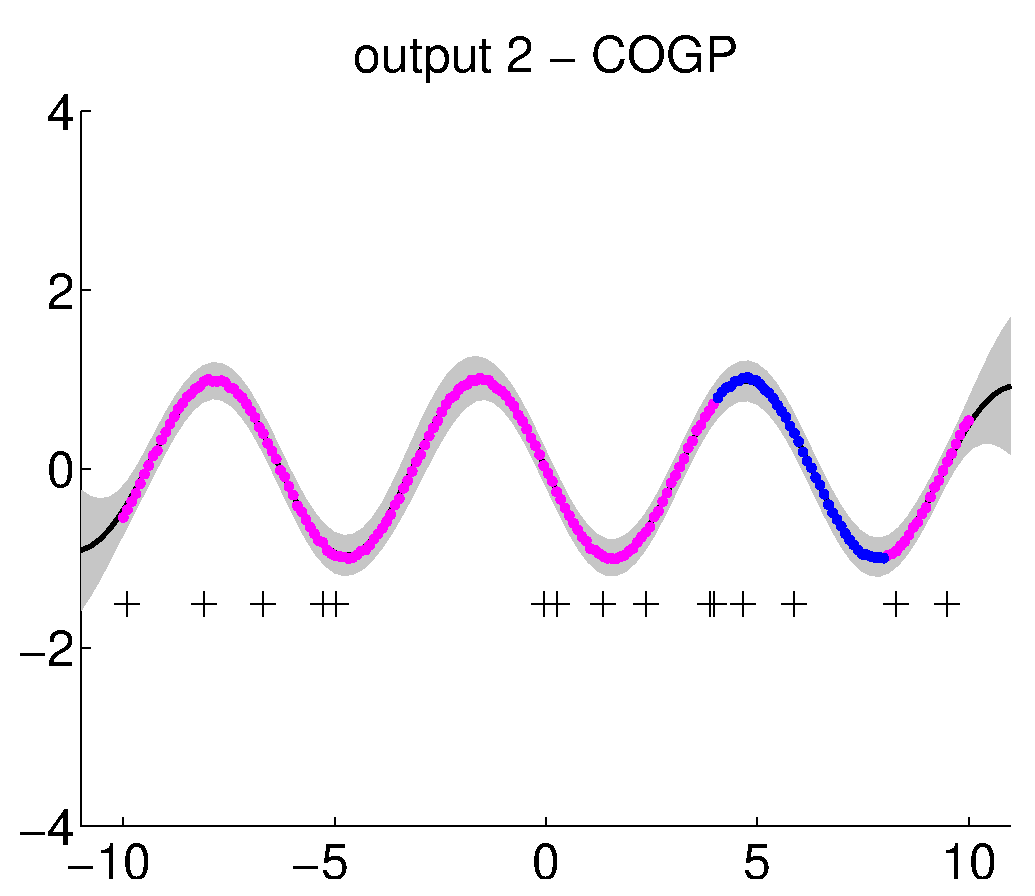
\includegraphics[scale=0.2]{figures/toy-slfm-y2.eps} &
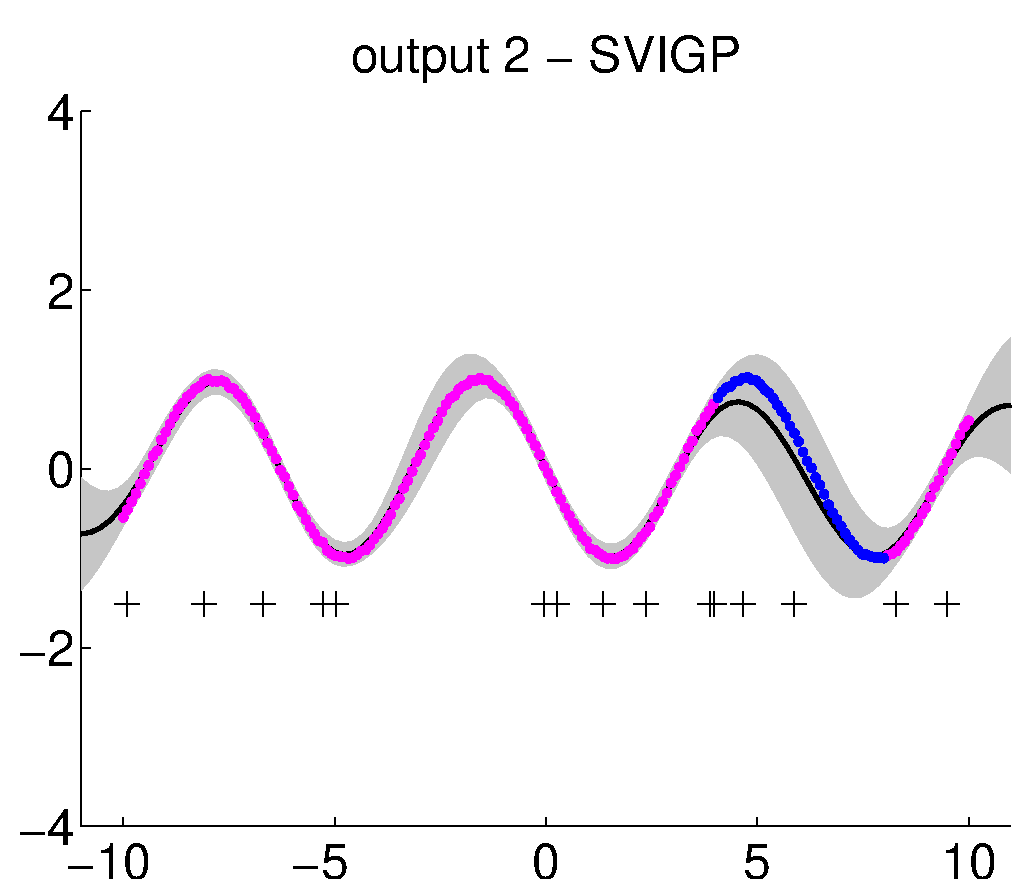
\includegraphics[scale=0.2]{figures/toy-svigp-y2.eps}
\label{fig:toy}
\end{tabular}
\caption{Predictive distributions of the multioutput GPs (first and third figure) and independent GPs using stochastic variational inference (second and last figure) for the  toy problem. Solid black line: predictive mean; grey bar: two standard deviations; magenta dots: real observations; blue dots: missing data. The black crosses show the locations of the inducing inputs.}
\label{fig:toy}
\end{figure*}

\subsection{FOREIGN EXCHANGE RATE PREDICTION}
The application considered here is to predict the foreign exchange rate w.r.t the US dollar of the top 10 international currencies (CAD, EUR, JPY, GBP, CHF, AUD, HKD, NZD, KRW, and MXN) and 3 precious metals (gold, silver, and platinum)\footnote{Data is available at http://fx.sauder.ubc.ca/data.html}. 
The setting of our experiment described here is identical to that in \citet{alvarez2010efficient}.
The dataset contains all the data available for the 251 working days in the year of 2007.
There are 9, 8, and 42 days of missing values  for gold, silver, and platinum, respectively.
We remove from the data the exchange rate of CAD on days 50-100, JPY on day 100-150, and AUD on day 150-200.
Note that these 3 currencies are from very different geographical locations. 
The 153 points extracted is used for testing and the remaining 3051 data points is used for training.
Since the missing data is long contiguous sections, the objective is to evaluate the capacity of the model to impute the missing currency values based on other currencies.
%todo: batch size, learn rate (maybe at the beginning of experiments)

For preprocessing we normalized the outputs to have zero mean and unit variance.
Since the exchange rates are driven by a small number of latent market forces \citet{alvarez2010efficient}, we tried different values of $Q = {1,2,3}$ and selected $Q = 2$ which gave the best model evidence (ELBO).
We used the squared-exponential covariance function for the shared processes and a noise covariance function for the independent process of each output.
The inducing inputs $(M = 100)$ are randomly selected from the training set and fixed throughout training.

The predictive distributions by our model (Figure \ref{fig:fx}) exhibit similar behavior to those by the convolved model with inducing kernels in \citet{alvarez2010efficient}.
In particular, both models perform better at capturing the strong depreciation of the AUD than the fluctuations of the CAD and JPY currency.
Our investigation of the dataset found that 4 other currencies (GBP, NZD, KRW, MXN) also experienced the same trend during the days 150 - 200.
This was effectively used by the model to extrapolate the values of the AUD.

%todo: result for independent gps
We also report in Table \ref{tab:fx} the predictive accuracy of our model compared to that of CGP variants and independent GPs. 
Our model outperforms both variants of the convolved GPs in terms of standardized mean-squared error (SMSE).
It has lower test likelihood, as measured by the negative log predictive density (NLPD), which is mainly due to the less conservative predictive variance of the full CGP for the CAD currency.
Note that the SMSE of CGPVAR is taken from \citet{alvarez2010efficient} while the NLPD was not provided.
Training took only 10 minutes for our model compared to 1.4 hours of the full CGP model.

\begin{table}[h]
\caption{Performance comparison on the foreign exchange rate dataset.}
\label{tab:fx}
\begin{center}
\begin{tabular}{c|c|c}
METHOD & SMSE & NLPD \\ \hline
COGP  & \textbf{0.2125} & -0.8394 \\
CGPVAR & 0.2795 & NA \\
CGP & 0.2427 & \textbf{-2.9474} \\
%ICM & 0.3927 &
\end{tabular}
\end{center}
\end{table}

\begin{figure*}
\centering
\begin{tabular}{ccc}
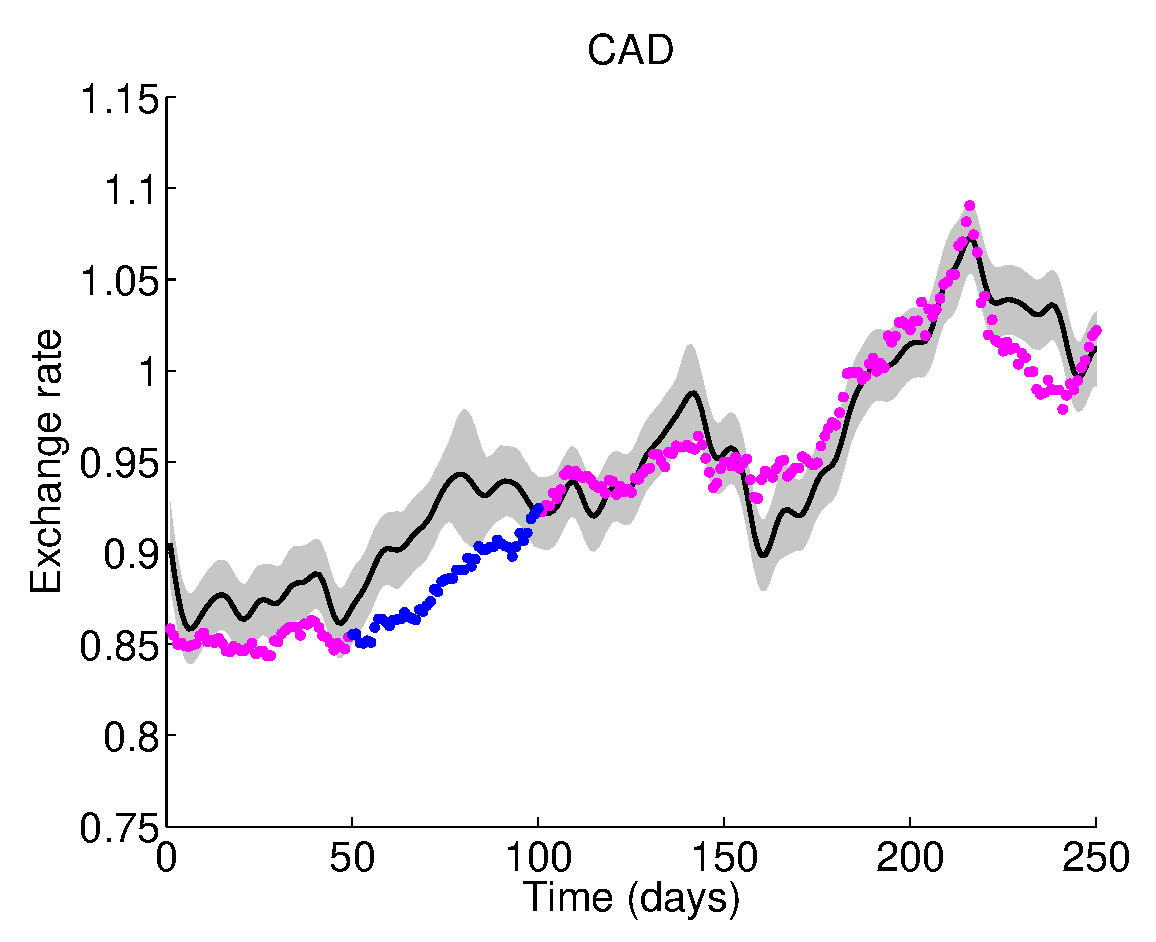
\includegraphics[scale=0.3]{figures/fxCAD.eps} &
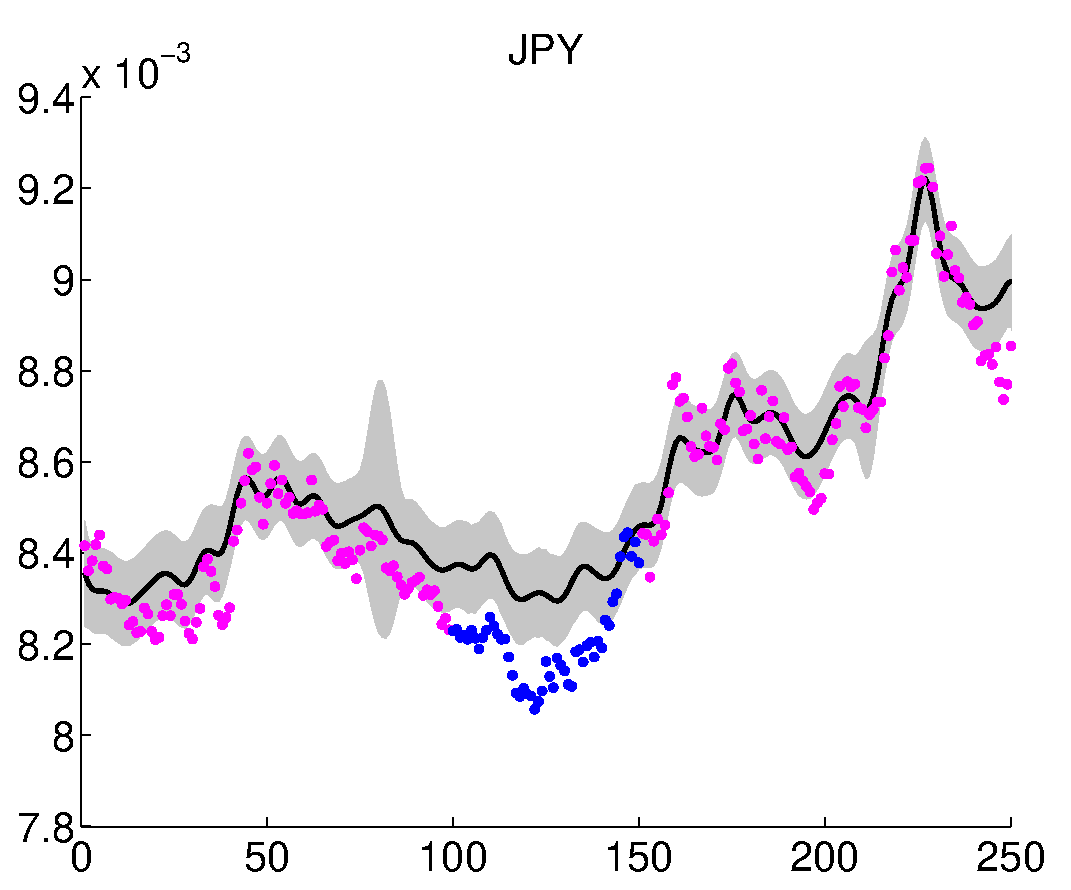
\includegraphics[scale=0.3]{figures/fxJPY.eps} &
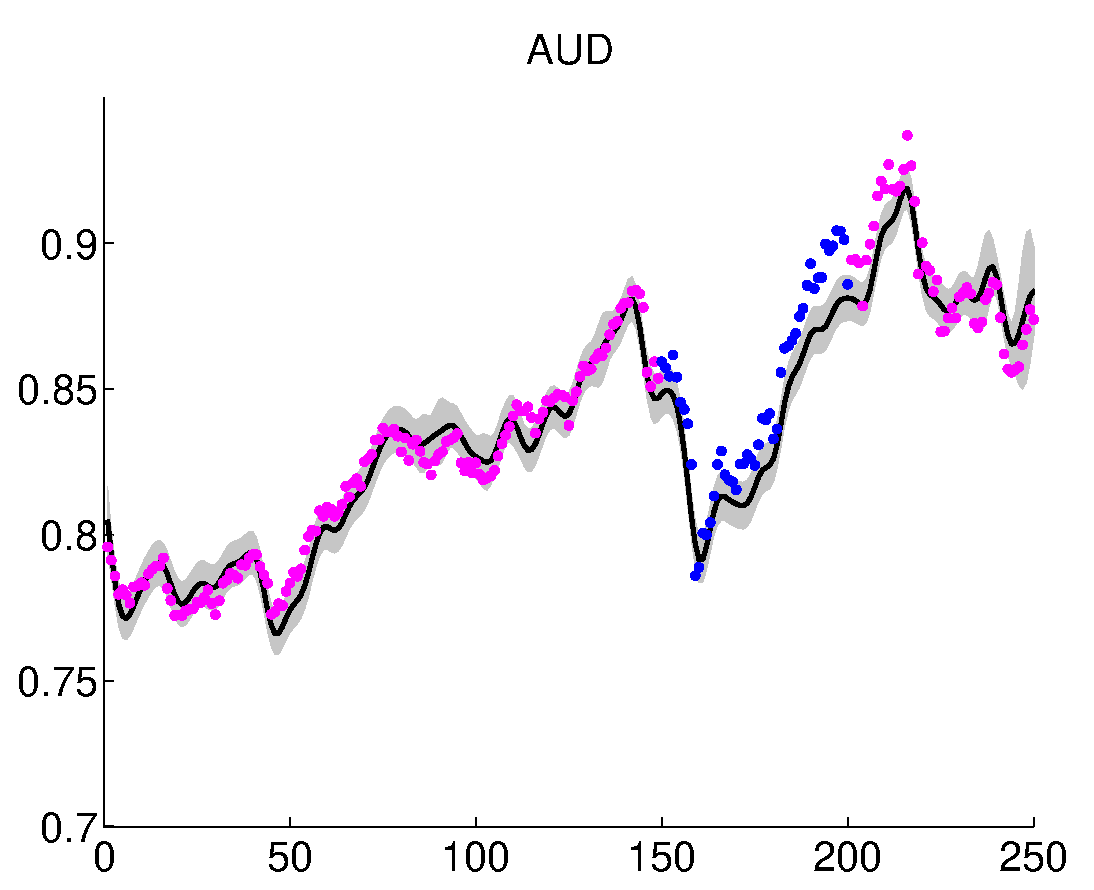
\includegraphics[scale=0.3]{figures/fxAUD.eps}
\end{tabular}
\caption{Real observations and predictive distributions for CAD (left), JPY (middle), and AUD (right). The color coding scheme is the same as in figure \ref{fig:toy}.}
\label{fig:fx}
\end{figure*}

\subsection{AIR TEMPERATURE PREDICTION}
Two latent functions, inverse lengthscale 136 capturing global trend of increasing temperature from day 10 - 15 and inverse lengthscale of 0.5 to model the fluctuation within a day.
Training for full cgp model with 2 latent functions took 3 hours compared to ... in our model.

\begin{table}[h]
\caption{Performance comparison by SMSE and NLPD on the air temperature dataset.}
\label{tab:fx}
\begin{center}
\begin{tabular}{c|c|c}
method & smse & nlpd \\ \hline
COGP & \textbf{0.1077} & \textbf{2.1712} \\
CGP & 0.1125 & 2.2219 \\
IGP & 0.8944 & 12.5319
\end{tabular}
\end{center}
\end{table}

\begin{figure*}
\centering
\begin{tabular}{ccc}
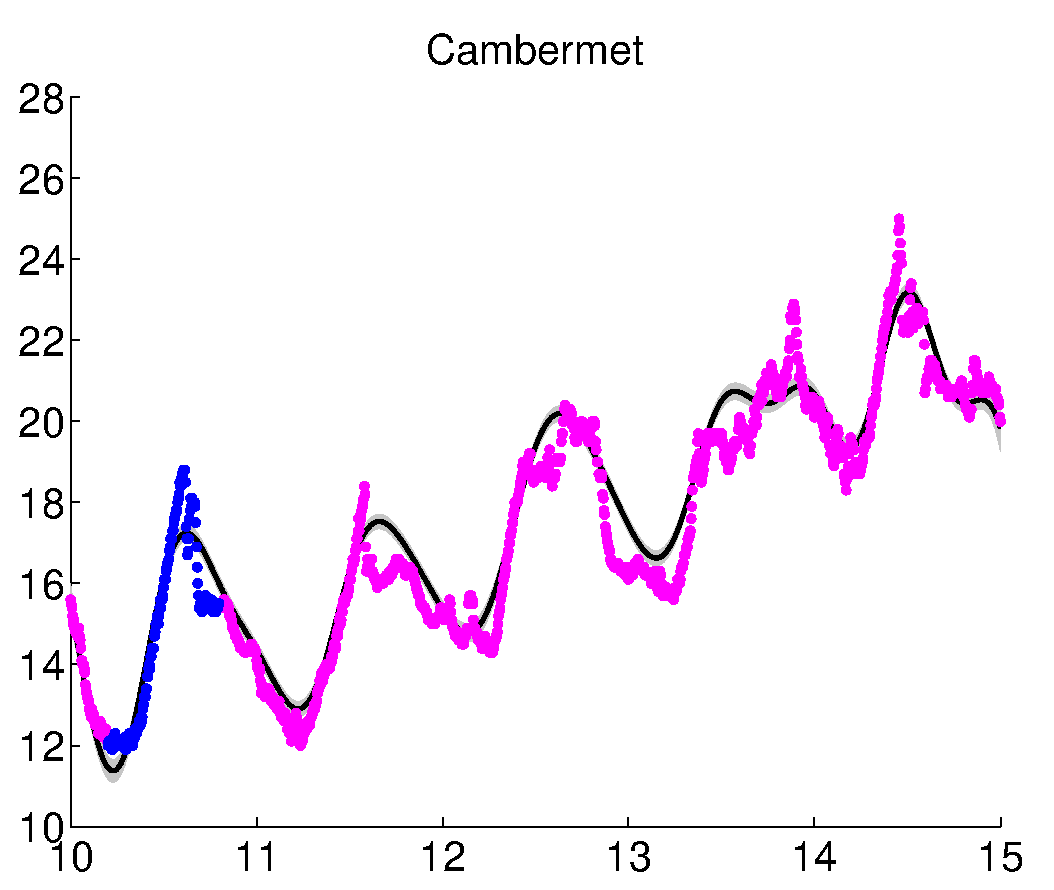
\includegraphics[scale=0.3]{figures/slfm-weatherCambermet.eps} &
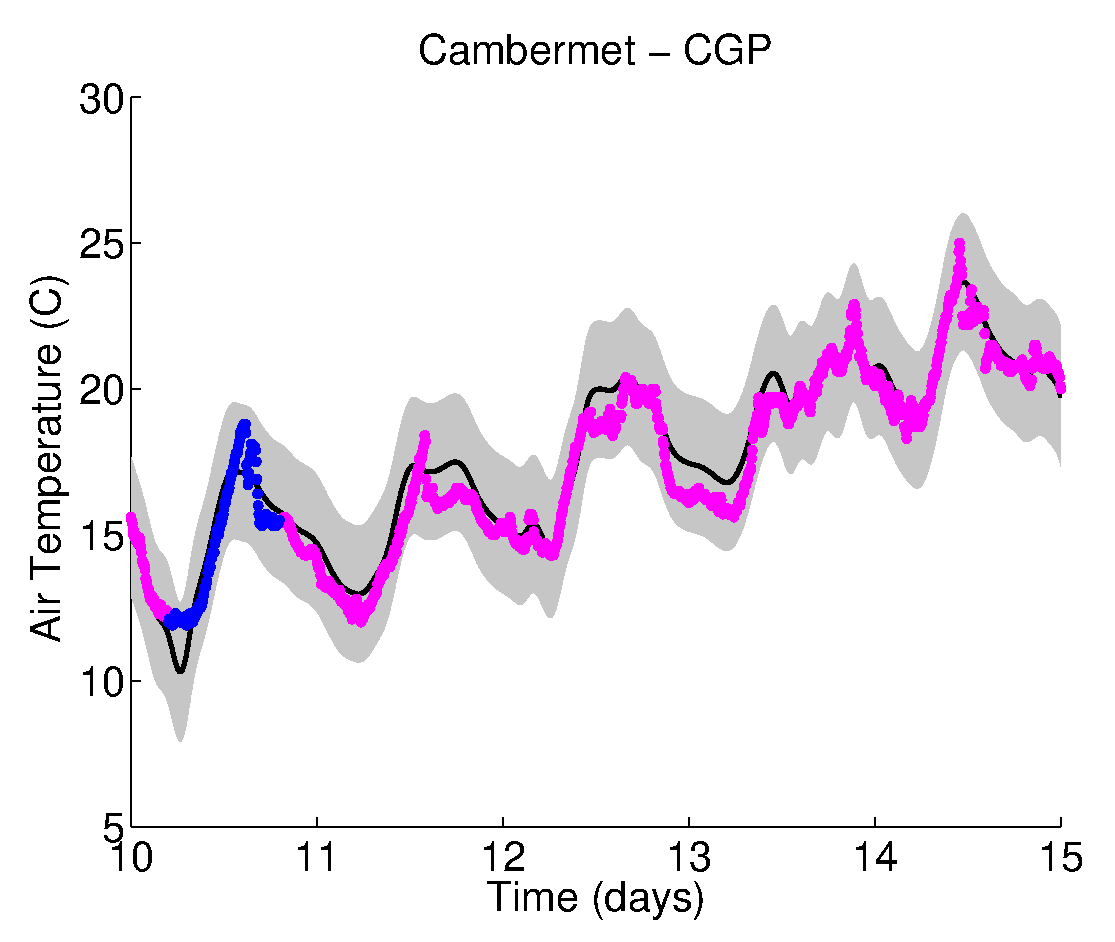
\includegraphics[scale=0.3]{figures/cgp-weatherCambermet.eps} &
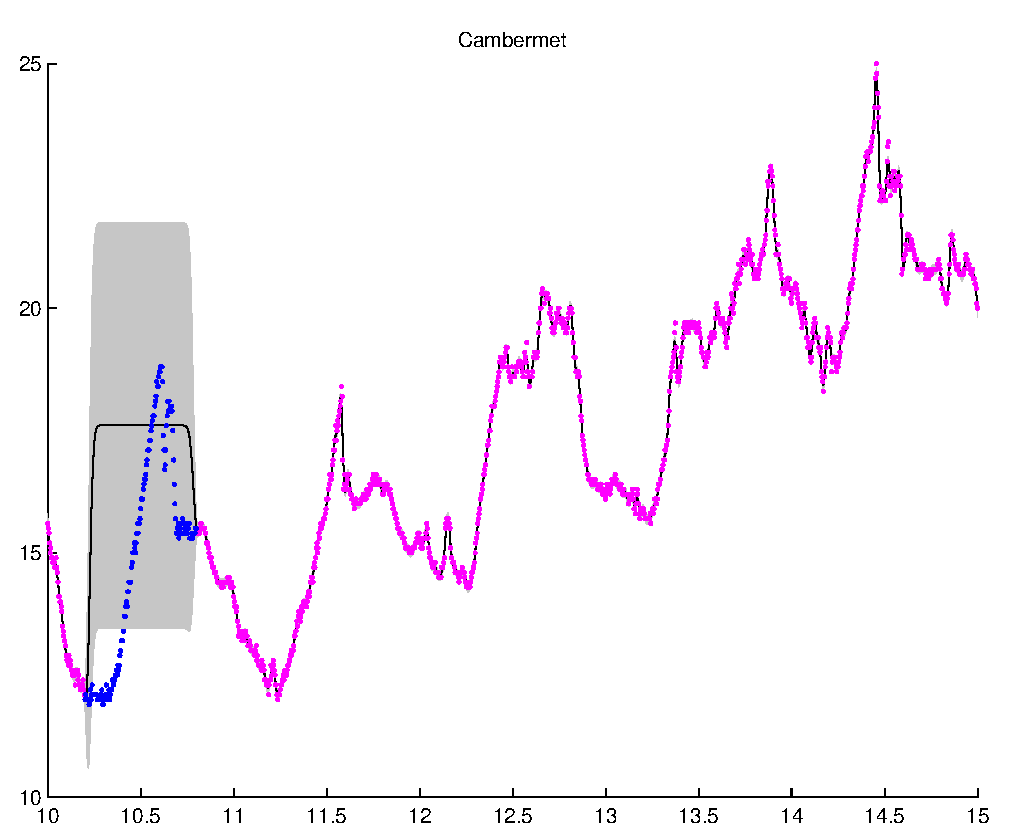
\includegraphics[scale=0.3]{figures/weatherCambermet.eps}
\\
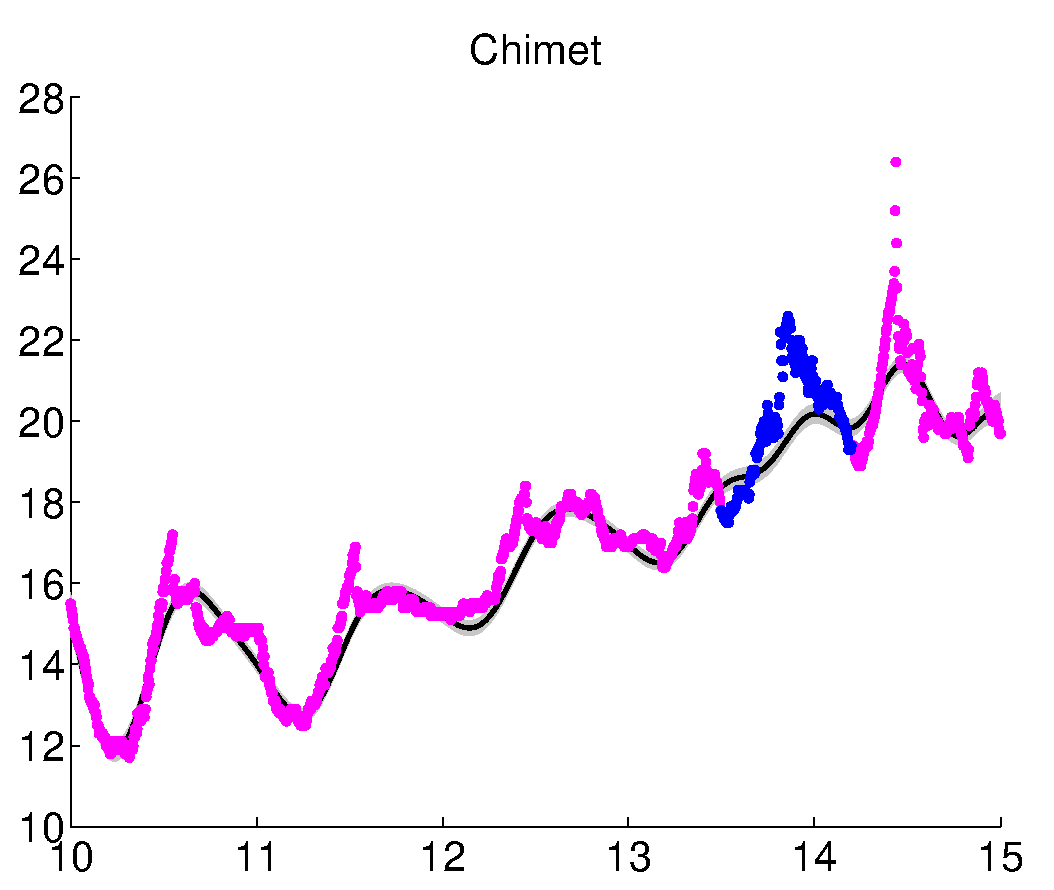
\includegraphics[scale=0.3]{figures/slfm-weatherChimet.eps} &
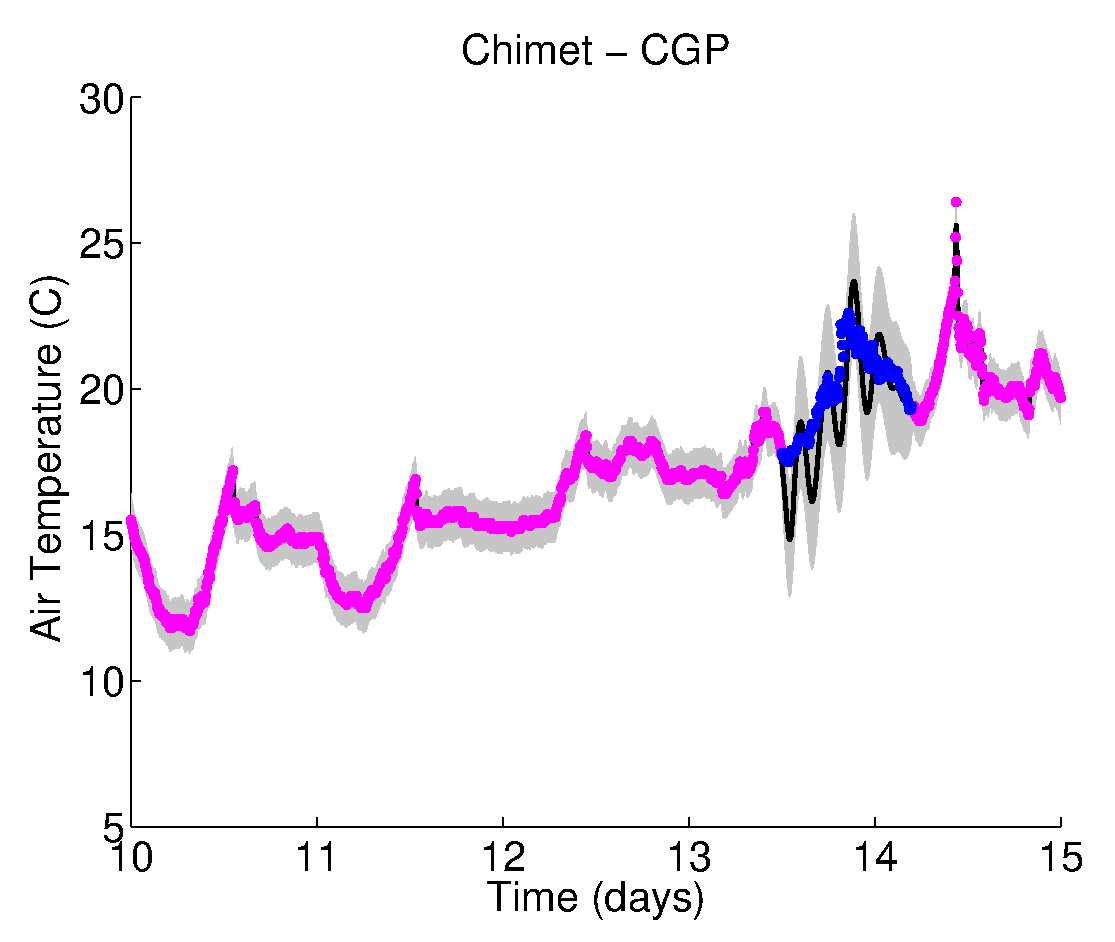
\includegraphics[scale=0.3]{figures/cgp-weatherChimet.eps} &
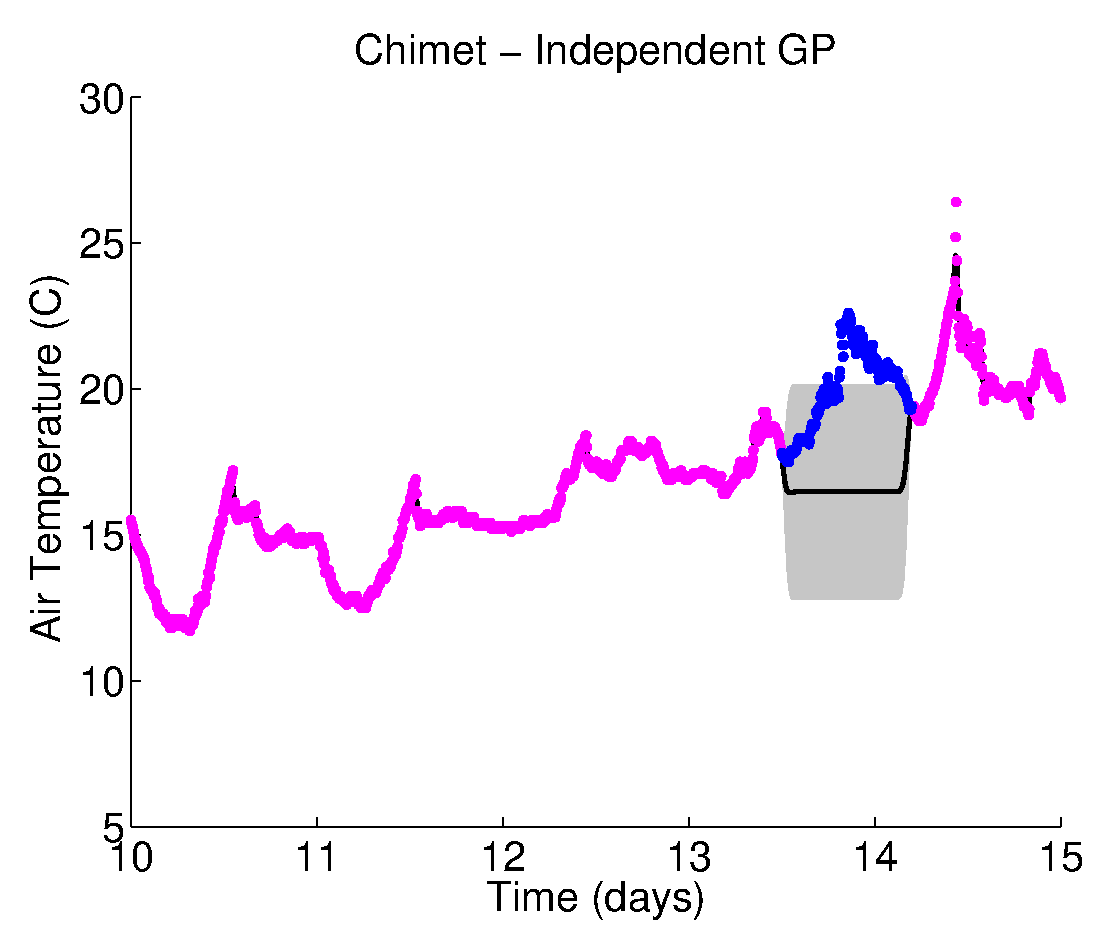
\includegraphics[scale=0.3]{figures/weatherChimet.eps}
\end{tabular}
\caption{Predictive distributions of the multioutput GPs (left column) and full independent GPs (right column) for the air temperature problem.}
\label{fig:weather}
\end{figure*}

\subsection{ROBOT ARMS}
